For our end goal of enabling large-scale autotuning, we need to explore the current capabilities and limitations of TVM first, especially with regard to the execution of multiple autotuning jobs simultaneously. The modern \gls{dl} landscape is very diverse in terms of models and hardware, so to evaluate TVM in a diverse range of scenarios is crucial for gaining a proper understanding. To this end, we developed a framework that enables us to a large number of experiments rapidly.

\section{SimpleTVM}
Since using TVM follows a similar flow every time, we created SimpleTVM which exposes the individual steps through a convenient interface. This makes it easy for researches who are new to TVM to get started. FSince a lot of the experiments include benchmarking, time measurements are taken for most steps and automatically saved in a \textit{benchmarking context}. The flow of SimpleTVM has some dependencies, which are enforced. For example, a model needs to be imported before building. The interface including possible flows is depicted in Figure \ref{fig:simpletvm-interface}. The methods that are exposes are now regarded closer.

\begin{figure}
	\centering
	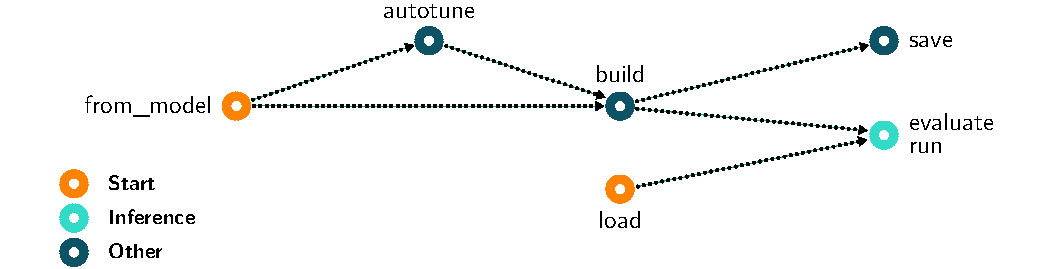
\includegraphics[width=\textwidth]{simpletvm_interface.pdf}%
	\caption{Interface and flow of SimpleTVM}
	\label{fig:simpletvm-interface}
\end{figure}

\begin{description}
	\item[\pythoninline/from_model/] Loading the Relay representation for the model is the beginning of a TVM flow. To that end, TVM supports the import from various frontends. Before the import of the model, however, it needs to be loaded and prepared for import. How exactly this is done differs even inside the same framework. SimpleTVM provides a unified import interface for TVM testing models, TensorFlow saved models (.pb files) and TensorFlow hub models. \pythoninline/from_model/ can easily be extended to support more frontends.
	\item[\pythoninline/autotune/] Once a model has been imported, autotuning can be run for each of the tensor operators. This step is optional, since TVM falls back to a default implementation if no records for that tensor operator exist in the autotuning database. Since this step is rather complex, there is a plethora of configuration options, the most important of which are exposed in \pythoninline/autotune/'s interface. SimpleTVM is designed to get new users started quickly so there are default values, but more experienced users can adjust the values according to their circumstances.
	\item[\pythoninline/build/] Before a TVM model can be executed, the target-specific executable needs to be build from the Relay model as described in the previous chapter. When building, SimpleTVM can either automatically use records from the global autotuning database, or the results from a specific autotuning job can be used.
	\item[\pythoninline/save/] After building, the library containing the operators can be saved along with the graph description and weights.
	\item[\pythoninline/load/] Beyond starting from an imported model, SimpleTVM can also load a previously saved TVM modules, which makes it possible to use a model that has been autotuned earlier. Saved modules can only be loaded if they have been built on the same device.
	\item[\pythoninline/run/] Inference can be run using this method. It accepts and returns a NumPy array. The input can, for example, be an image. However, loading the image and preparing it for inference, e.g., scaling and normalizing, needs to be done by the user.
	\item[\pythoninline/evaluate/] To profile the performance, \pythoninline/evaluate/ runs inference on random data multiple times, then averages the measured times. However, in contrast to the profiling stage of autotuning, not the performance of individual tensor operators but the whole model is measured.
\end{description}

An example of how SimpleTVM is typically used is presented in Listing \ref{lst:simpletvm-flow}. First, the \pythoninline/BenchmarkingContext/ is created (Line 1), which stores information about the current run such as the run id (a 32-character alphanumeric identifier for this execution of SimpleTVM), target device, measured times, the loaded model and the target device key to send to the tracker. When using a CPU as target device, the CPU architecture should be specified so TVM can select the proper hardware-specific tensor instructions. The benchmarking context is passed to the \pythoninline/SimpleTVM/ object (Line 2). Here, the address of the RPC tracker can be specified for distributed autotuning. If the address is not specified, autotuning will create a local tracker and server to perform autotuning on the same device as the client. Next, a model is imported (Line 3). Since the name of the output layer and the size of the output vector differs, it needs to specified explicitly. SimpleTVM's concise, chained syntax is used to autotune, build, save and evaluate the model (Line 4). For the sake of brevity, default parameters are leveraged, but the user can customize the actual calls to TVM functions by providing more parameters. Finally, the benchmarking context is saved (Line 5). This enables analysis at a later point, e.g., to examine the autotuning process or the inference performance measured by the evaluation. Note that this step is distinct from the saving of the TVM module. At a later point and usually by another application, the saved module which is identified by the run id can be loaded back. Then it can be used run inference on any data.

\begin{listing}
\begin{pythoncode}
ctx = BenchmarkingContext('cpu', device_key='i7', cpu_arch='skylake')
tvm = SimpleTVM(ctx, rpc_tracker=('tracker', 9190))
tvm.from_model('mobilenet.pb', output_name='out', output_size=10)
tvm.autotune().build().save().evaluate()
ctx.save()

# Saved model can be used later to run inference
tvm.load('run_id')
prediction = tvm.run(data)
\end{pythoncode}
\unskip
\caption{Typical SimpleTVM flow for CPU including autotuning}
\label{lst:simpletvm-flow}
\end{listing}

Additionally to SimpleTVM, we developed an automated benchmarking script called \textit{superb}. superb is short for \enquote{super benchmark} because it allows testing of different configurations without human intervention, so it performs benchmarking on a higher level than SimpleTVM's mechanisms. The user can specify the values for all parameters that should be tested. superb enumerates all possible combinations, effectively determining the $n$-ary product set of all value lists, then executes SimpleTVM once with each configuration. Additionally, it sets up the required servers and the tracker. The results from all configurations are collected and can then be processed by another script. This script evaluates the resulting inference performances, aggregates some information and writes them into a file, enabling further analysis with other tools such as Jupyter notebooks.

All SimpleTVM-related files are stored in the \enquote{\textasciitilde /.tvm-benchmark} directory. This includes the autotuning databases of currently running jobs, the global autotuning database and a file containing only the best known configurations. There are subdirectories for each SimpleTVM run with a log file for debugging, the saved benchmarking context and the autotuning log file for this run, if applicable. In another subdirectory, the results of superb experiments are collected with a csv file containing the aggregate information like mean autotuning time and the mean execution time for each stage. Finally, all saved modules are saved in a directory named after their run id.

Since we want to test TVM on a variety of machines, we created Docker images to be able to easily deploy TVM with all dependencies on any server. The \gls{gpu} version also includes the CUDA libraries, and a helper script for using the images mounts some folders into the container and sets up the environment. The Docker images in conjunction with SimpleTVM and superb form the foundation for our experiments.

\section{Parameters}
Autotuning with TVM offers a plethora of configuration options that affect both the autotuning process itself and the result. Setting these parameters to adequate values for the given job and hardware requires knowledge of how TVM works, but in some cases it is a matter of trial and error. However, guidelines and descriptions of the most important parameters can help. All of the following parameters can be specified when using SimpleTVM
\begin{description}
	\item[Number of trials] This determines the number of configurations to try for each autotuning task. A higher number will generally result in a better inference performance since the search space can be explored more, but this results in an increased autotuning completion time. However, the result starts to converge to the optimum after about 500 iterations, so there is a limit to the inference performance that can be achieved. Especially with CPUs, that have a small search space compared to \glspl{gpu}, there might not even be more options to try. Practically, the optimal result can be expected with the number of trials set to 2000.
	\item[Profiling timeout] This determines the time after which the profiling for one configuration is killed. Since every tensor operator has a different computational intensity and performance varies across types of hardware, this timeout needs to be adjusted accordingly. A high profiling timeout will allow longer execution, which drives up total autotuning completion time and might not yield better results since long-running implementations are not good and can safely be killed. A low profiling timeout might also kill of good implementations. It should be noted that the optimal timeout does not depend on the actual execution time, since profiling runs the implementation multiple times and might even dynamically adjust the number of executions. In practice, a low timeout should be set first. If the log shows too many timeout errors, the timeout can be increased. 5 seconds seems to be a good value for \gls{gpu} target devices, while 20 seconds or more are appropriate for CPU autotuning.
	\item[Batch size] This determines how many configurations are selected and built in parallel for every autotuning iteration. This can speed up autotuning considerably, especially if a large number of CPU cores are available on the client to run many compiler processes in parallel. The number of cores is also the default value. For larges batches, the model is updated and queried less frequently, but in general there seems to be no detrimental effect of having a high batch size. It should be notes that this is not the same as the batch size of the model, which would change the shape of the tensor operators.
	\item[Transfer learning] This determines whether or not transfer learning is used between jobs. According to this setting, the data from the global autotuning database might be used to train the cost model at the start of each task. Between tasks, there is always transfer learning. Usually, transfer learning should be enabled for the most optimal inference performance results. However, we disable transfer learning for experiments to guarantee a fair comparison between earlier and later ones.
\end{description}


\section{Capabilities}
Using SimpleTVM and our knowledge about proper parameter settings as foundation, we evaluated how TVM performs in comparison to state-of-the-art manual tensor operator libraries. We use TensorFlow 1.14 as baseline since it is a popular framework for \gls{dl} applications. cuDNN is enabled for \gls{gpu}. Autotuning with TVM was executed with 2000 trials, so the numbers should represent the optimal implementation. For evaluation, we test a Mobilenet with a batch size of on two mobile-grade CPUs (Intel Core i5-5300U and i5-7300U) and a server-grade \gls{gpu} (NVIDIA Tesla K80). Additionally, we test a heavier ResNet-18 on the \gls{gpu}.

\begin{figure}
	\centering
	\includegraphics[width=\textwidth]{chart_inference_tf_vs_tvm}%
	\caption{Inference performance with TensorFlow and TVM}
	\label{fig:inf-tf-tvm}
\end{figure}

Inference improvement vs default tvm and TF
Good in tradeoff with autotuning
Use numbers from paper and own numbers

\section{Limitations}
TVM suffers from some fundamental restrictions, which cannot be changed in the current design.

\subsection{Resource Utilization}
We noticed lots of resource idle time due to synchronous design
Show figure from poster
Want to minimize idle time because edge resources are limited (define edge)
Due to dependencies of stages, cannot be changed for a single job

\subsection{Scalability}
Our goal is to enable large-scale autotuning for our AaaS, autotune multiple models at the same time

objectives:
Be able to run an arbitrary number of autotuning jobs while
1. maximizing inference performance: ultimate goal of autotuning
2. minimize hardware requirements: save cost
3. minimizing autotuning time: make autotuning worth the effort
in order of priority
State that autotuning time is not as crucial since it is rendered negligible by a large amount of inferences

With default tvm, there are two possible setups
Include figure with two setups
Include table with three experiments here

1. two completely separate autotuning jobs running independently on additional dedicated servers, one autotuning runner per server
Pros: good autotuning and inference time, because they don't affect each other
Cons: Costly because we need multiple sets of the same hardware, bad hardware utilization
not an economically feasible approach. We cannot simply use machines from a PaaS provider since actual target device needs to be used
Alternatively, we could use the same server and run them in sequence, trading off hardware required (halved) for autotuning time(doubled)

2. two autotuning runners sharing the same server
Pros: only one set of hardware
Cons:
- interference drives up autotuning time
Explain interference
Autotuning takes long (in our tests anywhere between 3 and 36 hours, depending on hardware and network size)
Especially update model takes 64\% longer when two jobs are running simultaneously, very CPU intensive (50-70\%)
- results in worse inference performance because profiling is distorted (show numbers), as we saw most important

In both setups, we do not meet all objectives
Gets worse the more jobs we add
AaaS is not possible efficiently with current implementation and architecture of autotuning in TVM, does not scale well

Ideally:
Prevent interference, because it affects autotuning time and inference performance
Minimize hardware required by utilizing available hardware fully before adding new servers for cost reasons

However, there does not seem to be any solution yet

\subsection{Similar Problems}
In general, problem can be formulated as follows:
How can resources be shared optimally between multiple tasks that are partially idle?

Add two examples